\section{Ejemplos del lenguaje de marcado Latex}

Ths document is an example of BibTeX using in bibliography management. Three items 
are cited: \textit{The \LaTeX\ Companion} book \cite{latexcompanion}, the Einstein
journal paper \cite{einstein}, and the Donald Knuth's website \cite{knuthwebsite}. 
The \LaTeX\ related items are \cite{latexcompanion,knuthwebsite}\footnote{Esto está tomado de
\url{https://www.overleaf.com/learn/latex/Bibliography_management_with_bibtex}}.
 

  \textbf{Texto} en el párrafo 1.

  \textit{Texto} en el párrafo 2.

  \texttt{Texto} en el párrafo 3.


  \begin{itemize}
  \item Consideración 1
  \item Consideración 2
  \end{itemize}

  % Espacio vertical
  \vspace{0.5cm}
  
  \begin{enumerate}
  \item Punto 1
  \item Punto 2
  \end{enumerate}
  
A continuación se muestra una ecuación:

  \[ \int_{0}^{1}\frac{1}{x^2+1} dx \]

  Podemos incluir imágenes en formato: png, pdf o jpg.

  En la figura~\ref{fig:diagrama} se muestra un diagrama realizado con \href{yed}{https://www.yworks.com/products/yed}:

  \begin{figure}[!htb]
    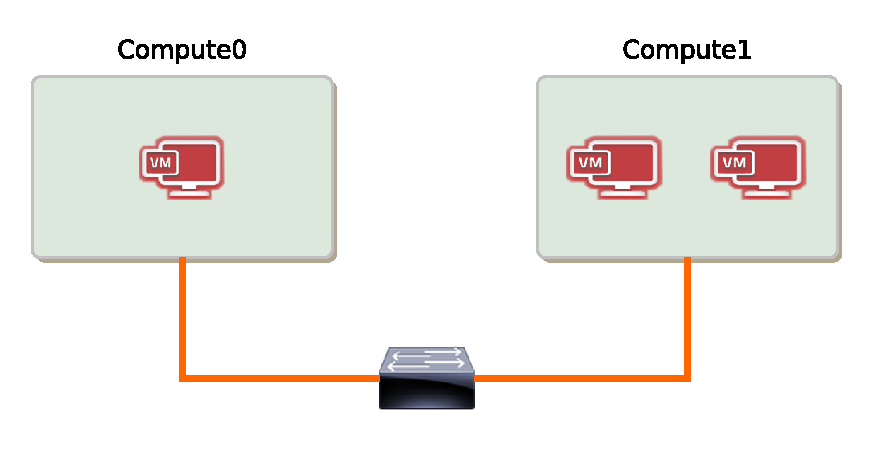
\includegraphics[width=0.8\textwidth]{diagrama.pdf}
    \caption{Esta es una figura que latex decide donde colocar (floating) en el documento.}
    \label{fig:diagrama}
    \end{figure}

  \begin{tabular}{cc}
    Imagen 1 & Imagen 2 \\[2mm]
    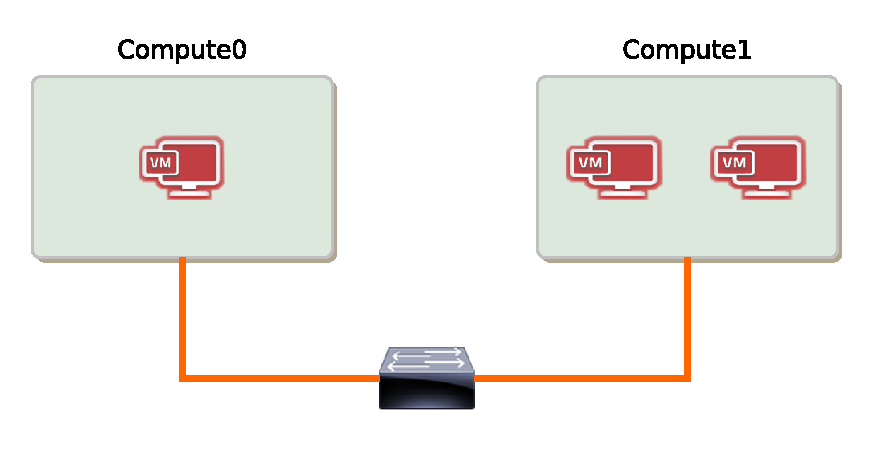
\includegraphics[width=0.4\textwidth]{diagrama.pdf} &  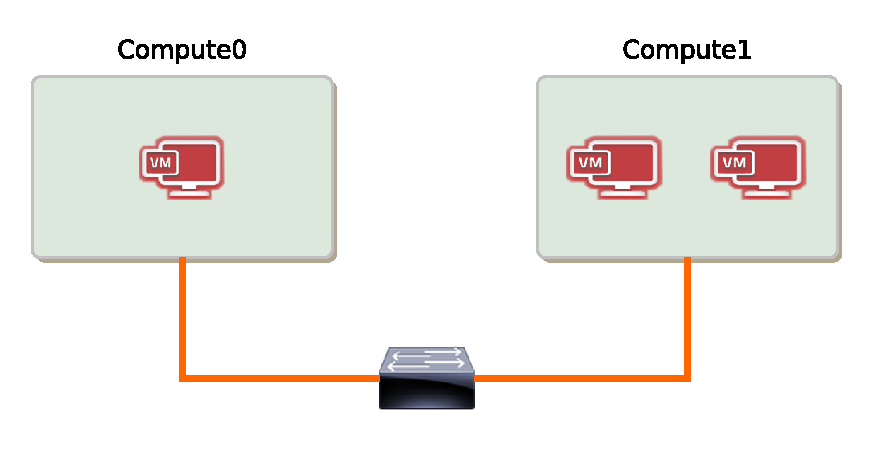
\includegraphics[width=0.4\textwidth]{diagrama.pdf}
  \end{tabular}
  
  Este es un ejemplo de una tabla:
  
  \begin{tabular}{|l|c|}
    \hline
    Columna 1 & Columna 2 \\ \hline
    1 & 2 \\ \hline
  \end{tabular}


  \vspace*{1cm}
  O la misma tabla centrada:

  \begin{center}
    \begin{tabular}{|l|c|}
      \hline
      Columna 1 & Columna 2 \\ \hline
      1 & 2 \\ \hline
    \end{tabular}
  \end{center}

  Para generar el fichero PDF:
  
  \begin{lstlisting}{language=bash}
    pdflatex ejemplo-memoria.tex
    bibtex ejemplo-memoria
    pdflatex ejemplo-memoria.tex
\end{lstlisting}

  También se puede usar \texttt{latexmk} que automáticamente regenera la bibliografía.
  \begin{lstlisting}{language=bash}
    latexmk -pdf ejemplo-memoria.tex
\end{lstlisting}

  